\documentclass[12pt, letterpaper]{book}

% Standard LaTeX Packages
\usepackage[utf8]{inputenc}
\usepackage[T1]{fontenc}
\usepackage{lmodern} % For better font quality
\usepackage{amsmath}
\usepackage{amssymb}
\usepackage{mathtools}
\usepackage{graphicx}
\usepackage{tikz} % Keep if diagrams are still needed
\usepackage{booktabs} % For professional quality tables
\usepackage{multicol} % If multicolumn layouts are still desired in some parts
\usepackage{xcolor} % For color definitions, if still needed
\usepackage{geometry} % For page layout
\usepackage{fancyhdr} % For custom headers and footers
\usepackage{hyperref} % For clickable links (TOC, references)

% Page geometry
\geometry{
    letterpaper,
    top=1in,
    bottom=1in,
    left=1.25in,
    right=1.25in,
    headheight=13.6pt
}

% Color definitions (if needed, or can be removed/modified)
\definecolor{mDarkTeal}{HTML}{23373b}
\definecolor{mLightBrown}{HTML}{EB811B}
\definecolor{mLightGreen}{HTML}{14B03D}

% Title information
\title{F1010 - Modeling with Differential Equations}
\author{Dr. Juliho Castillo\\julihocc@tec.mx}
\date{\today} % Or a specific date: June 8, 2025

% Header and Footer configuration
\pagestyle{fancy}
\fancyhf{} % Clear all header and footer fields
\fancyhead[LE]{\nouppercase{\leftmark}} % Chapter name on Left Even (outer)
\fancyhead[RO]{F1010 - Modeling with Differential Equations: A Comprehensive Text} % Book title on Right Odd (outer)
\fancyhead[RE,LO]{} % Clear inner headers
\fancyfoot[CE,CO]{\thepage} % Page number centered
\renewcommand{\headrulewidth}{0.4pt}
\renewcommand{\footrulewidth}{0.4pt}
\renewcommand{\chaptermark}[1]{\markboth{#1}{}}


\begin{document}

% Title page
\frontmatter % For parts like preface, TOC before main content
\maketitle

% Table of contents
\tableofcontents

\mainmatter % For main content chapters

\chapter{Introduction to the Course and Differential Equations}
\label{chap:introduction}

\section{Welcome to F1010}
\label{sec:welcome}

\subsection{Course Information}
\label{ssec:course_info}
\begin{itemize}
    \item \textbf{Course Code:} F1010
    \item \textbf{Course Title:} Modeling with Differential Equations
    \item \textbf{Credits:} 3-0-1-5.3-2-30-10-56-16-96-10-2
    \item \textbf{Discipline:} Physics
    \item \textbf{School:} Engineering and Sciences
    \item \textbf{Academic Department:} Sciences
    \item \textbf{Prerequisite:} MA1029
\end{itemize}

\subsection{Course Structure}
\label{ssec:course_structure}
\textbf{Session Organization:}
\begin{itemize}
    \item \textbf{Total Sessions:} 20 (conceptual, this is a book now)
    \item \textbf{Duration:} Equivalent to 2 hours each session
    \item \textbf{Contact Hours:} Equivalent to 40 hours
\end{itemize}

\textbf{Content Distribution (conceptual chapters/parts):}
\begin{itemize}
    \item 1 opening chapter/section (this one)
    \item 6 subject modules (covered in subsequent chapters)
    \item 1 comprehensive review/appendix (optional)
\end{itemize}

\section{Learning Objectives}
\label{sec:learning_objectives}
Upon completion of this course (and study of this book), you will be able to:

\begin{enumerate}
    \item \textbf{Define mathematical relations} between relevant physics variables of a system through fundamental principles.
    \item \textbf{Model the behavior of systems} through equations that describe the system's relevant quantities and rates of change.
    \item \textbf{Analyze reality based on facts} through inductive-deductive logical reasoning for problem-solving with valid, objective criteria.
\end{enumerate}

\section{Mathematical Prerequisites}
\label{sec:math_prereqs}

\subsection{MA1029 Concepts Review}
\label{ssec:ma1029_review}
Essential concepts from your prerequisite course:

\begin{multicols}{2}
\begin{itemize}
    \item Functions and their properties
    \item Limits and continuity
    \item Derivatives and differentiation rules
    \item Chain rule applications
    \item Implicit differentiation
    \item Integration techniques
    \item Fundamental Theorem of Calculus
    \item Parametric equations
    \item Polar coordinates
    \item Infinite series
\end{itemize}
\end{multicols}

\subsection{Quick Review: Derivatives}
\label{ssec:derivatives_review}
Basic differentiation rules:
\begin{align}
    \frac{d}{dx}[x^n] &= nx^{n-1} \label{eq:power_rule}\\
    \frac{d}{dx}[e^x] &= e^x \label{eq:exp_rule}\\
    \frac{d}{dx}[\sin x] &= \cos x \label{eq:sin_rule}\\
    \frac{d}{dx}[\ln x] &= \frac{1}{x} \label{eq:ln_rule}
\end{align}

The Chain Rule:
\begin{equation}
    \frac{d}{dx}[f(g(x))] = f'(g(x)) \cdot g'(x) \label{eq:chain_rule}
\end{equation}

\section{Introduction to Differential Equations}
\label{sec:intro_diff_eq}

What is a Differential Equation?
\newtheorem{definition}{Definition}[chapter] % Define a definition environment
\begin{definition}
    A \textbf{differential equation} is an equation that relates a function with one or more of its derivatives.
\end{definition}

Examples:
\begin{align}
    \frac{dy}{dx} &= 3x + 2 \quad &\text{(First-order ODE)} \label{eq:ex_first_order}\\
    \frac{d^2y}{dx^2} + 4y &= 0 \quad &\text{(Second-order ODE)} \label{eq:ex_second_order}\\
    \frac{\partial u}{\partial t} &= \frac{\partial^2 u}{\partial x^2} \quad &\text{(Partial Differential Equation - PDE)} \label{eq:ex_pde}
\end{align}

\subsection{Physical Significance}
\label{ssec:physical_significance}
Differential equations naturally arise in physics and engineering:
\begin{itemize}
    \item \textbf{Newton's Second Law:} $F = ma = m\frac{d^2x}{dt^2}$
    \item \textbf{Radioactive Decay:} $\frac{dN}{dt} = -\lambda N$
    \item \textbf{Population Growth:} $\frac{dP}{dt} = rP$
    \item \textbf{Heat Conduction:} $\frac{\partial T}{\partial t} = \alpha \nabla^2 T$
    \item \textbf{Wave Equation:} $\frac{\partial^2 u}{\partial t^2} = c^2 \frac{\partial^2 u}{\partial x^2}$
\end{itemize}
Differential equations are the language of change!

\subsection{Classification of Differential Equations}
\label{ssec:classification_de}
Differential equations can be classified in several ways:

\textbf{By Type:}
\begin{itemize}
    \item Ordinary Differential Equation (ODE): Contains derivatives with respect to only one independent variable.
    \item Partial Differential Equation (PDE): Contains partial derivatives with respect to two or more independent variables.
\end{itemize}

\textbf{By Order:}
The order of a differential equation is the order of the highest derivative present in the equation.
\begin{itemize}
    \item First-order (e.g., Equation~\ref{eq:ex_first_order})
    \item Second-order (e.g., Equation~\ref{eq:ex_second_order})
    \item Higher-order
\end{itemize}

\textbf{By Linearity:}
A differential equation is linear if the dependent variable and its derivatives appear only to the first power and are not multiplied together. Otherwise, it is non-linear.
\begin{itemize}
    \item Linear
    \item Non-linear
\end{itemize}

\textbf{By Coefficients:}
\begin{itemize}
    \item Constant coefficients: The coefficients of the terms involving the dependent variable and its derivatives are constants.
    \item Variable coefficients: At least one coefficient is a function of the independent variable.
\end{itemize}

\section{Mathematical Modeling}
\label{sec:math_modeling}

\subsection{The Modeling Process}
\label{ssec:modeling_process}
The process of mathematical modeling can be visualized as follows:
\begin{center}
    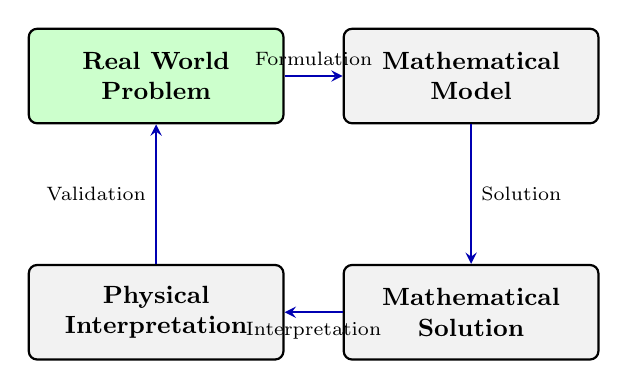
\begin{tikzpicture}[
        node distance=3cm and 2.5cm, % Adjusted distance
        auto,
        box/.style={
            draw,
            rectangle,
            rounded corners=3pt,
            text width=3cm, % Adjusted width
            text centered,
            minimum height=1.2cm, % Adjusted height
            fill=gray!10, % Generic fill
            draw=black,
            thick,
            font=\small\bfseries
        },
        arrow/.style={
            ->,
            thick,
            color=blue!70!black, % Generic arrow color
            >=stealth
        },
        label/.style={
            font=\scriptsize,
            color=black
        }
    ]
        \node (real) [box, fill=green!20] {Real World\\Problem};
        \node (math) [box, right of=real, node distance=4cm] {Mathematical\\Model}; % Increased node distance
        \node (solution) [box, below of=math, node distance=3cm] {Mathematical\\Solution};
        \node (interpret) [box, left of=solution, node distance=4cm] {Physical\\Interpretation}; % Increased node distance

        \draw[arrow] (real) -- (math) node[midway, above, label] {Formulation};
        \draw[arrow] (math) -- (solution) node[midway, right, label] {Solution};
        \draw[arrow] (solution) -- (interpret) node[midway, below, label] {Interpretation};
        \draw[arrow] (interpret) -- (real) node[midway, left, label] {Validation};
    \end{tikzpicture}
\end{center}

\subsection{Modeling Principles}
\label{ssec:modeling_principles}
Key steps in mathematical modeling:
\begin{enumerate}
    \item \textbf{Identify} the variables and parameters.
    \item \textbf{Make assumptions} to simplify the problem.
    \item \textbf{Formulate} the differential equation(s).
    \item \textbf{Solve} the equation(s) (analytically or numerically).
    \item \textbf{Interpret} the solution in physical terms.
    \item \textbf{Validate} against experimental data or known facts.
    \item \textbf{Refine} the model if necessary.
\end{enumerate}

\subsection{Example: Population Growth Model}
\label{ssec:example_population_growth}
\textbf{Problem:} Model the growth of a population over time.

\textbf{Assumptions:}
\begin{itemize}
    \item The birth rate is proportional to the current population.
    \item There are no deaths, immigration, or emigration (closed system).
    \item Resources are unlimited.
\end{itemize}

\textbf{Mathematical Model:}
Let $P(t)$ be the population at time $t$, and $r$ be the constant growth rate.
The rate of change of the population, $\frac{dP}{dt}$, is proportional to $P(t)$:
\begin{equation}
    \frac{dP}{dt} = rP \label{eq:population_growth}
\end{equation}
This is a first-order, linear, ordinary differential equation with constant coefficients.

\chapter{Further Topics (Placeholder)}
\label{chap:further_topics}
This chapter will cover the subsequent modules as outlined in the original course structure.

\section{First-Order Differential Equations}
(Content from Sessions 2-4 would go here)

\section{Second-Order Differential Equations}
(Content from Sessions 5-7 would go here)

% ... and so on for other modules ...

\appendix
\chapter{Assessment Framework (Conceptual)}
\label{app:assessment}
While this book serves as a textual resource, the original course assessment was structured as:
\begin{itemize}
    \item \textbf{50\% Cumulative Theoretical-Practical Midterm Examinations}
    \begin{itemize}
        \item After modules 2, 4, and 6 (sessions 7, 13, 19)
    \end{itemize}

    \item \textbf{20\% Activities, Assignments, and Integrating Cases}
    \begin{itemize}
        \item During practice sessions (4, 7, 10, 13, 16, 19)
    \end{itemize}

    \item \textbf{30\% Final Integrating Examination}
    \begin{itemize}
        \item Session 20 (comprehensive assessment)
    \end{itemize}
\end{itemize}
For self-study, readers are encouraged to work through examples and exercises provided in each chapter.

\chapter{Recommended Texts and Further Reading}
\label{app:texts}
\textbf{Primary Text (basis for much of this material):}
\begin{itemize}
    \item Nagle, R. Kent, Saff, Edward B., Snider, Arthur David. \textit{Fundamentals of Differential Equations and Boundary Value Problems}, 9th ed. Pearson, 2018. (Updated from original reference)
\end{itemize}

\textbf{Supplementary References:}
\begin{itemize}
    \item Simmons, George F. \textit{Differential Equations with Applications and Historical Notes}, 3rd ed. CRC Press, 2017.
    \item Boyce, William E., DiPrima, Richard C., Meade, Douglas B. \textit{Elementary Differential Equations and Boundary Value Problems}, 11th ed. Wiley, 2017.
    \item Zill, Dennis G. \textit{A First Course in Differential Equations with Modeling Applications}, 11th ed. Cengage Learning, 2018.
\end{itemize}

\backmatter % For bibliography, index, etc.
% \bibliography{references} % If you have a .bib file
% \bibliographystyle{plain}

% Placeholder for a simple bibliography if not using BibTeX
\begin{thebibliography}{9}
    \bibitem{nagle2018} Nagle, R. K., Saff, E. B., \& Snider, A. D. (2018). \textit{Fundamentals of Differential Equations and Boundary Value Problems} (9th ed.). Pearson.
    \bibitem{simmons2017} Simmons, G. F. (2017). \textit{Differential Equations with Applications and Historical Notes} (3rd ed.). CRC Press.
    \bibitem{boyce2017} Boyce, W. E., DiPrima, R. C., \& Meade, D. B. (2017). \textit{Elementary Differential Equations and Boundary Value Problems} (11th ed.). Wiley.
    \bibitem{zill2018} Zill, D. G. (2018). \textit{A First Course in Differential Equations with Modeling Applications} (11th ed.). Cengage Learning.
\end{thebibliography}

\end{document}
